\section{System Design}\label{sec:sysdesign}

\begin{figure}[htpb]
\centering
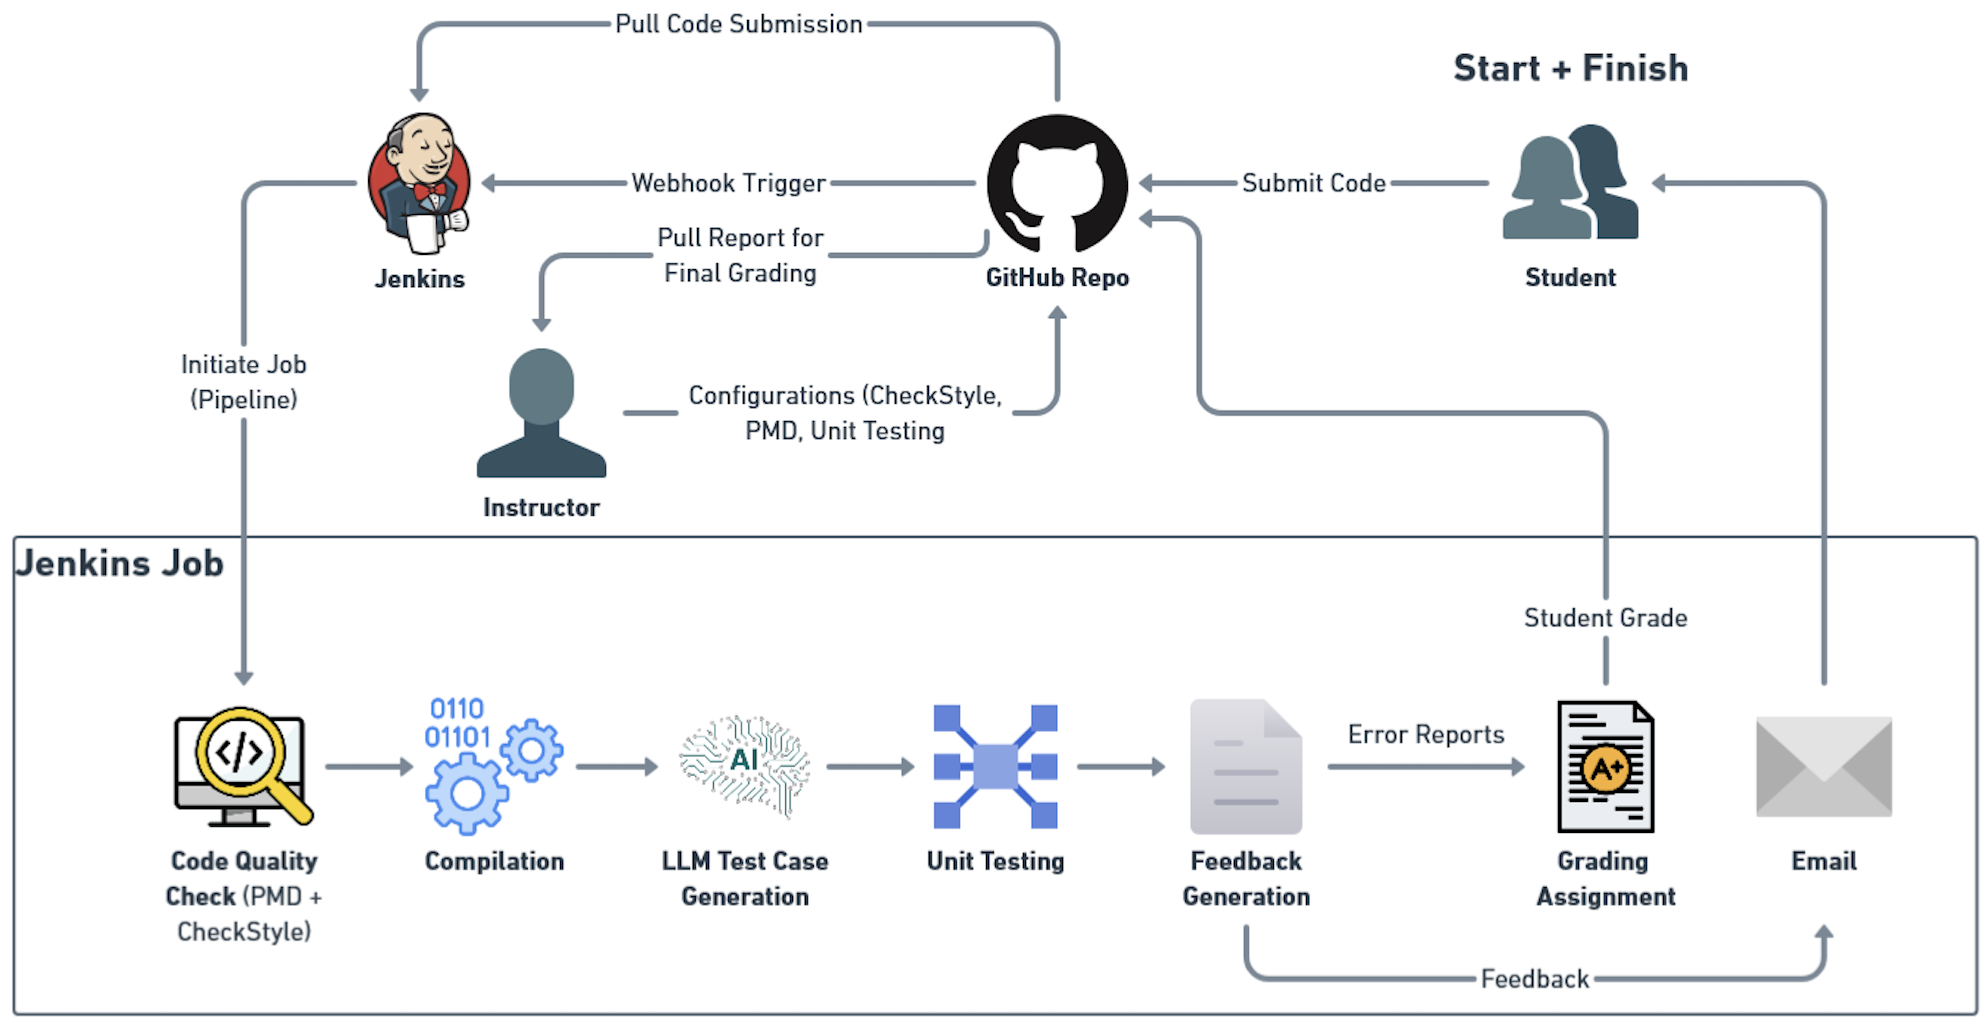
\includegraphics[width=
\linewidth]{fig/codeinspct.png}
\caption{\codeinspector design.}
\label{fig:codeinspector}
\end{figure}

Figure~\ref{fig:codeinspector} shows the architectural design of the proposed system. \codeinspector integrates Jenkins as its central component and LLM for test case generation. The workflow pipeline of the main components shown in the figure is discussed below.

\subsection{Code Submission}
\codeinspector offers a web-based front-end interface that allows students to submit their code for evaluation. Students upload their code as a Java file or write it directly using an integrated code editor. The code is then automatically submitted to the instructor's GitHub repository.

\subsection{Test Case Generation}\label{llm}
The system uses LLM to generate unit tests designed to evaluate the correctness of student code. We implemented an API using the Flask\footnote{https://flask.palletsprojects.com/en/stable/} framework, enabling communication between \codeinspector and the LLM. The open-source tool Ollama\footnote{https://ollama.com} executes the LLM locally, eliminating reliance on cloud-based processing. Specifically, we employ Meta's ollama3.2\footnote{https://www.llama.com/llama-downloads/}. LLaMA (Large Language Model Meta AI)~\cite{touvron2023llama} is a family of state-of-the-art open-weight LLMs that balance computational efficiency with advanced natural language processing capabilities, offering researchers and developers access to powerful AI tools without extensive computational resources. The API accepts a Java file containing an instructor's solution to a programming assignment. The LLM uses the file and a carefully designed prompt specifying rules to generate test cases using the JUnit framework. 
This process produces a Java file containing test cases for expected inputs and edge cases, which is returned to \codeinspector as the API response.

\subsection{Code Assessment}
When students commit their code to the instructor’s GitHub repository, GitHub triggers the Jenkins pipeline job for \codeinspectoren, thereby automating the entire assessment process. The pipeline then performs several steps to streamline the build and assessment process. First, it downloads dependencies to set up the execution environment. Next, it retrieves the student code from the GitHub repository, an Apache Ant script for build automation, and the LLM-generated test file. Finally, Jenkins executes the Ant script to compile the code, run unit testing against the executable, and perform the style analysis on the source code.

We selected the JUnit framework for black-box testing and used CheckStyle and PMD for code style analysis. Both CheckStyle and PMD are highly scalable and configurable, enabling instructors to select which checks should be considered when analyzing students' code. To ensure relevance, we configured these tools to enforce a small set of coding standards suitable for novice programmers. Due to space limitations, Table \ref{tab1} provides a very brief description of the coding standards from the grading rubric used for the Java code submissions; for a detailed description, see \cite{10590588,Imhmed2024fosterCQ}.

Additionally, PMD and CheckStyle enable instructors to customize style error severity levels. In PMD, severity is defined on a scale from 1 to 4, where one is the most severe, while in CheckStyle, severity levels are categorized as error, warning, or info. Once the unit test execution and code style analysis are complete, assessment reports are generated detailing the number of passed and failed tests and identified style errors categorized by severity.

\begin{table}[tbp]
    \caption{Coding standards grading criterion, from~\cite{10590588}.}
    \centering
    \begin{tabular}{l p{0.55\columnwidth}}
       \hline
       \textbf{\textit{Criterion}} & \textbf{\textit{Description}} \\  
       \hline
       \hline
       Javadoc Documentation & The code is well documented, including proper JavaDoc tags that comment on the author's name, date, program's task, and JavaDoc methods that effectively document the program's methods. \\
              %  \hline
       Comments & Comments specifying the objective of each method and control flow constructs are present and meaningful. \\
              %  \hline
       Naming Conventions & The program names, methods, and variables are descriptive and adhere to coding standards. \\
              %  \hline
       Whitespace & There is proper indentation and white space; code lines are not excessively long (less than 100 characters). \\
       \hline
    \end{tabular}
    \label{tab1}
\end{table}

\subsection{Feedback Generation}
At this stage, \codeinspector consumes the detailed reports generated from unit test execution and style analysis to create more formative feedback, which is then emailed to the corresponding student. This report lists aggregated counts of style errors by severity and details the first three detected errors, while hiding details of other violations until earlier errors are addressed. It also includes test case outcomes and an error-weighted density metric, providing students with insights into their performance relative to their peers.

By providing streamlined feedback via email, \codeinspector allows students to revise their code and resubmit it for further assessment. This structured approach minimizes cognitive overload, encourages incremental progress, and promotes iterative refinement rather than dependence. Moreover, it enables instructors to track student progress more efficiently.  Future improvements may include submission tokens to limit excessive resubmissions and reduce over-reliance on \codeinspector for debugging. 

\subsection{Automated Grading}
In the final stage of the Jenkins pipeline, \codeinspector grades student submissions using predefined, tiered criteria that range from Excellent to Unsatisfactory. A percentage threshold determines each tier and contributes a specific portion to the total grade for the corresponding criterion (see~\cite{10590588}). The grading criteria are outlined below.

\subsubsection{Requirements} This criterion evaluates how thoroughly the submitted code meets the assignment's functional requirements. The grade calculation for this criterion is straightforward. \codeinspector runs JUnit tests and then calculates the pass rate to determine which points should be assigned from the tiered rubric.

\subsubsection{Coding Standards}
Unlike the requirements criterion, style error distributions can vary significantly between submissions. To ensure fairness when grading this criterion, we adopt a penalty-based system rather than threshold scoring or simply counting total errors, thereby penalizing each style error according to its severity. Additionally, code size is considered since smaller or incomplete submissions may have fewer violations than larger ones. Penalizing solely based on total violations without considering code size is unfair and may discourage novice programmers from writing more extensive code to avoid higher penalties. Therefore, our grading method bases penalties on error-weighted density rather than total violations.

\begin{algorithm}[tbp]
        \fontsize{8pt}{8pt}\selectfont
        \SetAlgoLined
        \KwIn{Max\_Grade, Min\_Grade, Max\_Deduction, Penalty\_per\_Category, Errors\_per\_Category, LOC}
        \KwOut{Final\_Grade}
              Let Total\_Penalty $\leftarrow$ 0\;
                     
                     \ForEach{category $\in$ Errors\_per\_Category[category]}
              {
              Absolute\_Penalty $\gets$ Penalty\_per\_Category[category] $\times$ Errors\_per\_Category[category]\;
              Error\_Density $\gets$ Errors\_per\_Category[category] $\div$ {LOC}\;
              Adjusted\_Penalty $\gets$ Absolute\_Penalty $\times$ Error\_Density\;
              Total\_Penalty $\gets$ Total\_Penalty + Adjusted\_Penalty\;
              }

              Final\_Grade $\gets$ max(Max\_Grade - min(Total\_Penalty, Max\_Deduction), Min\_Grade)\;
        \KwRet{Final\_Grade}\;
        \caption{Error-weighted density grading.}
        \label{algo1}
\end{algorithm}

% Algorithm \ref{algo1} implements the grading scheme used by \codeinspector to determine the code quality grade of a submission. The process begins by computing the absolute penalty for each error category, calculated as the total style violations multiplied by the corresponding penalty weight. Next, the algorithm calculates the error density to normalize the penalty relative to code size; error density is defined as the number of errors per line of code (LOC). The adjusted penalty is then obtained by scaling the absolute penalty by the error density, ensuring that students with larger codebases are not unfairly penalized for having more violations. This adjusted penalty is then subtracted from the maximum grade, with the deduction capped at a maximum limit to prevent excessive penalties. Finally, the resulting grade is compared to a predefined minimum threshold, and the higher value is assigned as the student’s final grade, ensuring that grades do not fall below this minimum.

Algorithm \ref{algo1} implements the grading scheme used by \codeinspector to determine the code quality grade of a submission. The process begins by computing the absolute penalty for each error category, calculated as the total style violations multiplied by the corresponding penalty weight. Next, the algorithm calculates the error density to normalize the penalty relative to code size; error density is defined as the number of errors per line of code (LOC). Each category’s adjusted penalty is then obtained by scaling the absolute penalty by the error density, ensuring that students with larger codebases are not unfairly penalized for having more violations. The total penalty is calculated by summing the adjusted penalties and is then subtracted from the maximum grade, with the deduction capped at a maximum limit to prevent excessive penalties. Finally, the resulting grade is compared to a predefined minimum threshold, and the higher value is assigned as the student’s final grade, ensuring that grades do not fall below this minimum.

\subsubsection{Runtime}
Like the requirements criterion, \codeinspector runs unit and edge case tests to assess the code’s correctness and behavior. The grade assigned from the grading rubric corresponds directly to the test pass rate.